\documentclass{article}

\usepackage{graphicx}
\usepackage{tikz}
\usepackage{tikzsymbols}
\usetikzlibrary{calc,patterns,shapes.geometric}
\pagestyle{empty}
\usepackage[margin=0pt]{geometry}
\geometry{papersize={14in,12in}}

\def\centerarc[#1](#2)(#3:#4:#5){\draw[#1] ($(#2)+({#5*cos(#3)},{#5*sin(#3)})$) arc (#3:#4:#5);}

\begin{document}
	\begin{figure}
		\centering
		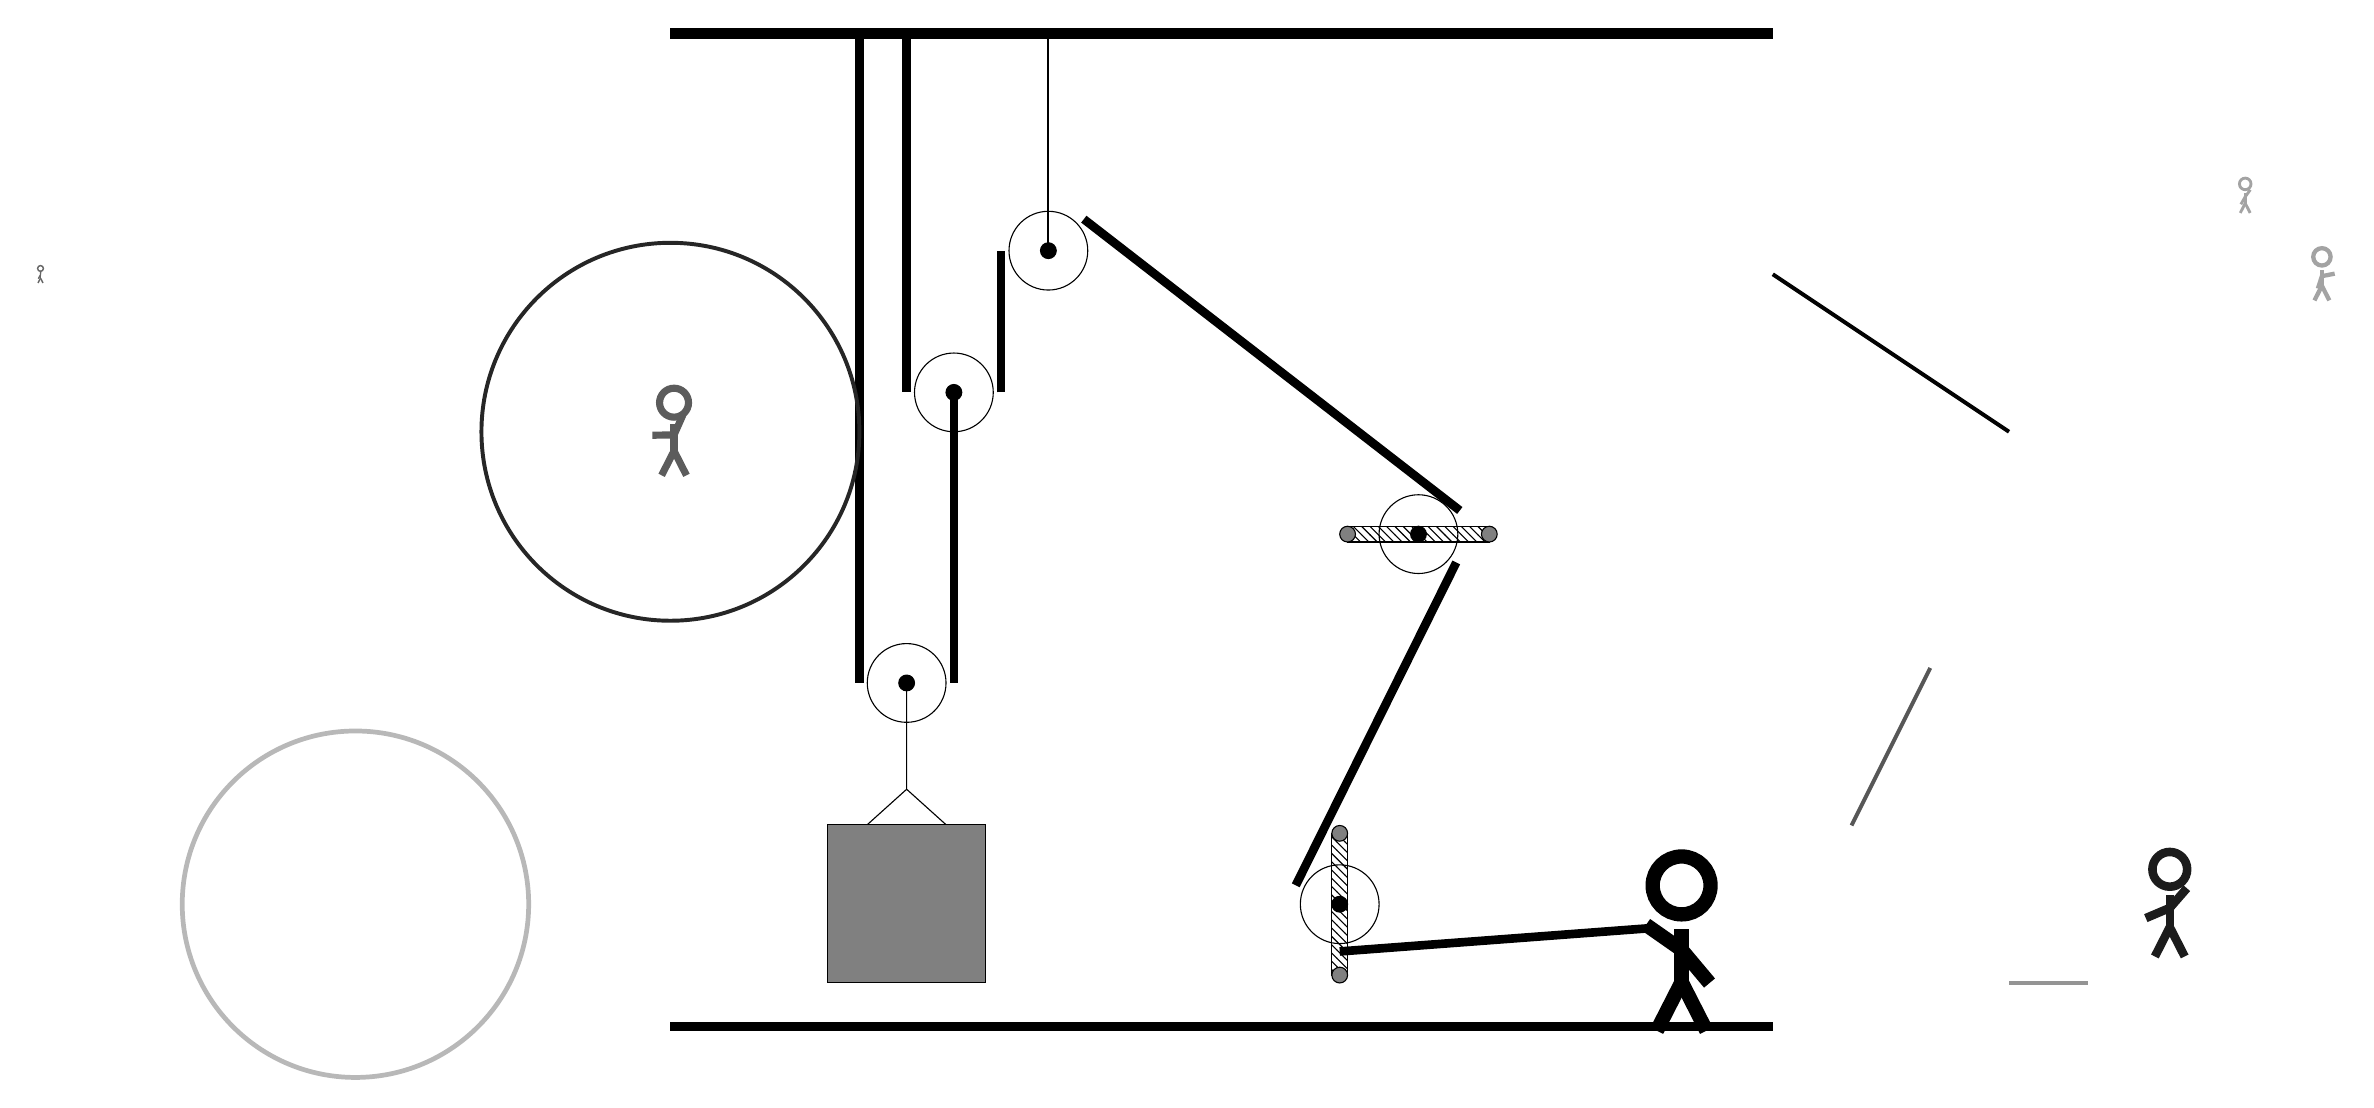
\begin{tikzpicture}
			%%%%% START %%%%%
			
			\draw[fill=black] (-2, 9) rectangle (12, 9.125);
			
			\draw (1, 0.81) circle (0.5);
			\draw[fill=black] (1, 0.81) circle (0.1);
			
			\draw (1.6, 4.5) circle (0.5);
			\draw[fill=black] (1.6, 4.5) circle (0.1);
			
			\draw (2.8, 6.3) circle (0.5);
			\draw[fill=black] (2.8, 6.3) circle (0.1);
			\draw[thick] (2.8, 6.3) -- (2.8, 9);
			
			\draw (6.5, -2) circle (0.5);
			\draw[fill=black] (6.5, -2) circle (0.1);
			\draw[pattern=north west lines, pattern color=black] (6.4, -1.1) rectangle (6.6, -2.9);
			\draw[fill=black!50] (6.5, -1.1) circle (0.1);
			\draw[fill=black!50] (6.5, -2.9) circle (0.1);
			
			\draw (7.5, 2.7) circle (0.5);
			\draw[fill=black] (7.5, 2.7) circle (0.1);
			\draw[pattern=north west lines, pattern color=black] (6.6, 2.8) rectangle (8.4, 2.6);
			\draw[fill=black!50] (6.6, 2.7) circle (0.1);
			\draw[fill=black!50] (8.4, 2.7) circle (0.1);
			
			\draw (1, 0.81) -- (1, -0.54) -- (0.5, -0.99) -- (1.5, -0.99) -- (1, -0.54);
			\draw[fill=black!50] (0, -0.99) rectangle (2, -2.99);
			
			\draw[line width=1.1mm] (0.4, 9) -- (0.4, 0.81);
			\centerarc[line width=1.1mm](1, 0.81)(180:360:0.6);
			\draw[line width=1.1mm](1.6, 0.81) -- (1.6, 4.5);
			\draw[line width=1.1mm] (1.0, 9) -- (1.0, 4.5);
			\centerarc[line width=1.1mm](1.6, 4.5)(180:360:0.6);
			\draw[line width=1.1mm](2.2, 4.5) -- (2.2, 6.3);
			\centerarc[line width=1.1mm](2.8, 6.3)(35:180:0.6);
			\draw[line width=1.1mm] (3.25, 6.7) -- (8.025, 3.0);
			\centerarc[line width=1.1mm](7.5, 2.7)(215:135:-0.6);
			\draw[line width=1.1mm](7.98, 2.34) -- (5.942, -1.76);
			\centerarc[line width=1.1mm](6.5, -2)(-30:100:-0.6);
			\draw[line width=1.1mm](6.5, -2.6) -- (10.5, -2.3);
			
			\node at (10.8, -2.5) {\Strichmaxerl[10][-35][-50]};
			
			\draw[line width=0.5mm, color=black!66](14, 1) -- (13, -1);
			
			\node[line width=0.7mm, color=black!60] at (-10, 6) {\Strichmaxerl[1][60][89]};
			\draw [line width=0.6mm, color=black!28](-6, -2) circle (2.2);
			\node[line width=0.7mm, color=black!36] at (19, 6) {\Strichmaxerl[3][72][11]};
			
			\draw[line width=0.5mm, color=black!42](15, -3) -- (16, -3);
			\draw [line width=0.5mm, color=black!85](-2, 4) circle (2.4);
			\node[line width=0.3mm, color=black!36] at (18, 7) {\Strichmaxerl[2][60][54]};
			
			\node[line width=0.6mm, color=black!89] at (17, -2) {\Strichmaxerl[6][23][49]};
			\draw[line width=0.5mm, color=black!99](12, 6) -- (15, 4);
			\node[line width=0.2mm, color=black!64] at (-2, 4) {\Strichmaxerl[5][1][66]};
			
			\draw[fill=black] (-2, -3.5) rectangle (12, -3.6);
			
			%%%%% END %%%%%
		\end{tikzpicture}
	\end{figure}	
\end{document}